\documentclass[11pt]{article}

% packages
\usepackage{physics}
% margin spacing
\usepackage[top=1in, bottom=1in, left=0.5in, right=0.5in]{geometry}
\usepackage{hanging}
\usepackage{amsfonts, amsmath, amssymb}
\usepackage[none]{hyphenat}
\usepackage{fancyhdr}
\usepackage[nottoc, notlot, notlof]{tocbibind}
\usepackage{graphicx}
\graphicspath{{./images/}}
\usepackage{float}
\usepackage{siunitx}
\usepackage{esint}
\usepackage{cancel}

% header/footer formatting
\pagestyle{fancy}
\fancyhead{}
\fancyfoot{}
% define a new page style called firststyle
\fancypagestyle{firststyle}{
\fancyhead[L]{MAC3474 Calculus III Honors Dr. Shabanov - Final Exam}
\fancyhead[R]{Sai Sivakumar - MetalNinja 25007801}
\fancyfoot[R]{\thepage/$6$}
}
\fancyfoot[R]{\thepage/$6$}
\renewcommand{\headrulewidth}{0pt}

% paragraph indentation/spacing
\setlength{\parindent}{0cm}
\setlength{\parskip}{5pt}
\renewcommand{\baselinestretch}{1.25}

% extra commands defined here
\newcommand{\ihat}{\boldsymbol{\hat{\textbf{\i}}}}
\newcommand{\jhat}{\boldsymbol{\hat{\textbf{\j}}}}
\newcommand{\dr}{\vec{r}~^{\prime}(t)}
\newcommand{\dx}{x^{\prime}(t)}
\newcommand{\dy}{y^{\prime}(t)}

\newcommand{\br}[1]{\left(#1\right)}
\newcommand{\sbr}[1]{\left[#1\right]}
\newcommand{\cbr}[1]{\{#1\}}

\newcommand{\dprime}{\prime\prime}
\newcommand{\lap}[2]{\mathcal{L}[#1](#2)}

% bracket notation for inner product
\usepackage{mathtools}

\DeclarePairedDelimiterX{\abr}[1]{\langle}{\rangle}{#1}

% set page count index to begin from 1
\setcounter{page}{1}

\begin{document}
\thispagestyle{firststyle}
I have opted to TeX this exam due to the increase in time given, since it would improve legibility and also my ability to check my work.

\textbf{1*}. The vector field $\mathbf{F}$ contains components that are all polynomials, so it is everywhere defined and its partial derivatives exist everywhere. Then to check if $\mathbf{F}$ is conservative we take its curl and find that it is the zero vector:
$$\nabla \times \mathbf{F} = \det \begin{pmatrix}
    \hat{\mathbf{e}}_1 & \hat{\mathbf{e}}_2 & \hat{\mathbf{e}}_3 \\
    \frac{\partial}{\partial x} & \frac{\partial}{\partial y} & \frac{\partial}{\partial z} \\
    2x-yz & 4y-xz & 6z-xy
\end{pmatrix} = \left\langle (-x)-(-x), (-y)-(-y) ,(-z)-(-z) \right \rangle = \mathbf{0}$$

Hence $\mathbf{F}$ is conservative over the whole space. This means that line integrals taken within this vector field possess the path independence quality, and so we may use the Fundamental Theorem for Line Integrals. We must construct the potential function $f(x,y,z)$ for this gradient field:
$$\pdv{f}{x} = 2x-yz \to f(x,y,z) = x^2-xyz + g(y,z)$$
$$\pdv{f}{y} = 4y-xz = \pdv{g}{y}-xz \to \pdv{g}{y} = 4y \to g(y,z) = 2y^2 + h(z) \to f(x,y,z) = x^2-xyz + 2y^2 + h(z)$$
$$\pdv{f}{z} = 6z-xy = \dv{h}{z} - xy \to \dv{h}{z} = 6z \to h(z) = 3z^2 + C$$
$$\to f(x,y,z) = x^2 + 2y^2 + 3z^2 -xyz + C$$

The contour (call it $C$) given in the problem begins at $(0,0,0)$ and ends at $(1,1,1)$, and by the fundamental theorem for line integrals we may simply evaluate the potential function at these terminal points to find the value of the line integral over the given contour $C$.
$$\int_C \mathbf{F}\cdot \dd{\mathbf{r}} = f(1,1,1) - f(0,0,0) = \br{(1) + 2(1) + 3(1) -(1) + C} - \br{C}$$
$$\boxed{= 5}$$

\noindent\makebox[\linewidth]{\rule{19.1cm}{0.4pt}}

\textbf{2*}. The surface (flux) integral we are trying to evaluate is $$\iint_S \mathbf{F} \cdot \hat{\mathbf{n}} \dd{S}$$ where $S$ is the surface given by $g(x,y) = z = xy$ where $x$ and $y$ are restricted to the annular region $D$ given by $1 \leq x^2+y^2 \leq 4$. Due to how the Jacobian of transformation is computed for surface integration, the following is true:
$$\iint_S \mathbf{F} \cdot \hat{\mathbf{n}} \dd{S} = \iint_D \mathbf{F} \cdot \mathbf{n} \dd{A}, ~ \mathbf{n} = \left\langle -g^{\prime}_x, -g^{\prime}_y ,1 \right \rangle = \left\langle -y, -x ,1 \right\rangle$$

Evaluate $\mathbf{F}$ on points $(x,y,g(x,y))$ and use polar coordinates ($1 \leq r \leq 2$, $0 \leq \theta < 2\pi$) to evaluate the integral:
$$\iint_D \left\langle x^2y, xy^2 , xy \right\rangle \cdot \left\langle -y, -x ,1 \right\rangle \dd{A} \to \iint_D \br{-2x^2y^2 + xy}\dd{A}$$
$$ \to \int_0^{2\pi}\int_1^2 \br{-2r^4\cos^2(\theta)\sin^2(\theta) + r^2\cos(\theta)\sin(\theta)}r\dd{r}\dd{\theta} $$
$$\to \int_0^{2\pi}\br{\frac{-2\br{2^6-1}}{6}\br{\frac{1}{4}\sin^2(2\theta)} + \cancel{\frac{2^4-1}{4}\br{\frac{1}{2}\sin(2\theta)}}}\dd{\theta} \to \frac{-21}{4}\int_0^{2\pi}\frac{1}{2}\br{1-\cancel{\cos(4\theta)}}\dd{\theta}$$
$$\boxed{=\frac{-21\pi}{4}}$$

\noindent\makebox[\linewidth]{\rule{19.1cm}{0.4pt}}

\textbf{3*}. Applying Green's theorem directly we find
$$\oint_C \br{\ln(x^2)+a^2y^3}\dd{x} + \br{e^{y^2}-b^2x^3}\dd{y} = \iint_D \br{-3b^2x^2 - 3a^2y^2} \dd{A}$$ where $D$ is the region enclosed by $C$.

The change of coordinates from $D$ to a new circular region $D^{\prime}$ is given by $x = au$, $y = bv$, whose Jacobian of transformation that satisfies $\dd{x}\dd{y} = J\dd{u}\dd{v}$ is found like so:
$$J = \det \begin{pmatrix}
    a & 0 \\
    0 & b
\end{pmatrix} = ab$$

Proceed with the computation, using geometry to evaluate the final integral:
$$\iint_D \br{-3b^2x^2 - 3a^2y^2} \dd{A} \to \iint_{D^{\prime}} \br{-3b^2a^2u^2 - 3a^2b^2v^2} ab \dd{A^{\prime}}$$
$$\to -3a^3b^3\iint_{D^{\prime}} \br{1} \dd{A^{\prime}}$$
$$\boxed{= -3a^3b^3\pi}$$

\noindent\makebox[\linewidth]{\rule{19.1cm}{0.4pt}}

\textbf{4*}. By the double angle identity $\sin(2t) = 2\sin(t)\cos(t)$, we find that the parametric closed curve lies on the surface given by $g(x,y) = z = 2xy$, and encloses a smooth surface $S$ that is part of $g(x,y)$. Furthermore, the vector field $\mathbf{F}$ contains components that are analytic in the whole space, so we can use Stokes' theorem to simplify the line integral like so:
$$\oint_C \mathbf{F}\cdot \dd{\mathbf{r}} = \iint_S \br{\nabla \times \mathbf{F}}\cdot \hat{\mathbf{n}} \dd{S} = \iint_D \br{\nabla \times \mathbf{F}}\cdot \mathbf{n} \dd{A}$$

The planar region $D$ is the unit disk, as that is enclosed by the projection of the curve $C$ into the $xy$ plane, $\left\langle \cos(t), \sin(t), 0 \right\rangle$.

Compute the curl of the vector field:
$$\nabla \times \mathbf{F} = \det \begin{pmatrix}
    \hat{\mathbf{e}}_1 & \hat{\mathbf{e}}_2 & \hat{\mathbf{e}}_3 \\
    \frac{\partial}{\partial x} & \frac{\partial}{\partial y} & \frac{\partial}{\partial z} \\
    y+\sin(x) & z^2+\cos(y) & x^3
\end{pmatrix} = \left\langle -2z, -3x^2 ,-1 \right \rangle$$

Then find the normal vector (oriented upward since the curve is oriented in the positive sense relative to viewing the curve from above the surface) to the surface $g(x,y) = z = 2xy$:
$$\mathbf{n} = \left\langle -g^{\prime}_x, -g^{\prime}_y ,1 \right\rangle = \left\langle -2y, -2x ,1 \right\rangle$$

Substitute into the simplified form of the integral and evaluate using geometry:
$$\iint_D \eval{\left\langle -2z, -3x^2 ,-1 \right \rangle \cdot \left\langle -2y, -2x ,1 \right\rangle}_{z = 2xy} \dd{A} \to \iint_D \br{\cancel{8 x y^2 + 6x^3} -1} \dd{A}$$

The first two terms provide no contribution to the integral due to symmetry over the $y$ axis ($x\to -x$). The integral evaluates to: $$\boxed{-\pi}$$

\noindent\makebox[\linewidth]{\rule{19.1cm}{0.4pt}}

\textbf{5*}. The components of the vector field $\mathbf{F}$ are polynomials and so are defined everywhere, and also have partial derivatives everywhere. This means we can use the divergence theorem. Say $E$ is the solid region bounded by the sphere $S$ defined by $x^2 + y^2+ z^2 = 2x$.

By the divergence theorem (written for when the normal vector points inwards), we can change the flux integral like so:
$$\oiint_S \mathbf{F}\cdot (-1)\hat{\mathbf{n}}\dd{S} = -\iiint_E \br{\nabla \cdot \mathbf{F}} \dd{V}$$

The divergence of $\mathbf{F}$ is:
$$\pdv{x}\br{x^3-x^2+yz} + \pdv{y}\br{y^3+xz^5} + \pdv{z}\br{z^3-x^2y^6} = 3x^2-2x+3y^2+3z^2$$

Then define spherical coordinates in the manner where the $x$ axis is the vertical axis:
$$x = \rho \cos(\phi), ~ y = \rho\sin(\phi)\cos(\theta), ~ z = \rho \sin(\phi)\sin(\theta)$$

From the equation of the sphere given, find that $$x^2 + y^2+ z^2 = 2x \to \rho^{2} = 2\rho\cos(\phi) \to \rho = 2\cos(\phi)$$

Then bounds in spherical coordinates for the region $E$ are $0\leq \rho \leq 2\cos(\phi)$, $0\leq \phi \leq \frac{\pi}{2}$, $0\leq \theta < 2\pi$. So the triple integral in terms of these spherical coordinates is computed like so:
$$-\int_0^{2\pi}\int_0^{\frac{\pi}{2}}\int_0^{2\cos(\phi)}\br{3\br{\rho \cos(\phi)}^2-2\br{\rho \cos(\phi)}+3\br{\rho\sin(\phi)\cos(\theta)}^2+3\br{\rho \sin(\phi)\sin(\theta)}^2}\br{\rho^2\sin(\phi)}\dd{\rho}\dd{\phi}\dd{\theta}$$
$$\to -\int_0^{2\pi}\int_0^{\frac{\pi}{2}}\int_0^{2\cos(\phi)}\br{3\rho^4 \sin(\phi)\cos^2(\phi)-2\rho^3 \sin(\phi)\cos(\phi)+3\rho^4\sin^3(\phi)\cos^2(\theta)+3\rho^4 \sin^3(\phi)\sin^2(\theta)}\dd{\rho}\dd{\phi}\dd{\theta}$$
$$\to -2\pi\int_0^{\frac{\pi}{2}}\int_0^{2\cos(\phi)}\br{3\rho^4 \sin(\phi)\cos^2(\phi)-2\rho^3 \sin(\phi)\cos(\phi)+3\rho^4\sin(\phi)\sin^2(\phi)}\dd{\rho}\dd{\phi}$$
$$\to -2\pi\int_0^{\frac{\pi}{2}}\int_0^{2\cos(\phi)}\br{3\rho^4 \sin(\phi)-2\rho^3 \sin(\phi)\cos(\phi)}\dd{\rho}\dd{\phi}$$
$$\to -2\pi\int_0^{\frac{\pi}{2}}\br{\frac{96}{5} \sin(\phi)\cos^5(\phi)-\frac{40}{5} \sin(\phi)\cos^5(\phi)}\dd{\phi}$$
$$\to 2\pi \int_0^1 \br{-\frac{56}{5} u^5}\dd{u} = 2\pi\br{\frac{-56}{30}}$$
$$\boxed{= -\frac{56}{15}\pi}$$

Because the flux turned out to be negative for this negatively oriented closed surface, there is a \textbf{faucet} within the sphere.

\noindent\makebox[\linewidth]{\rule{19.1cm}{0.4pt}}

\textbf{6*}. The vector field $\mathbf{F}$ has components that are polynomials, except the first component involves a tangent term which still has partial derivatives that exist because we are not dealing with $z$ values at $\pm \frac{\pi}{2}$, just between $0$ and $1$.

The deformation of the surface that works is to add on the unit disk oriented downwards (to match the outward orientation of the cone, give its unit normal vector as $-\hat{\mathbf{e}}_3$) lying in the $xy$ plane, as when $z=0$, $x^2+y^2 = 1$. Call the surface of the cone $C$ and then the disk $S$, then call the region bounded by $C\cup S$ as $E$. Then the following is true by the divergence theorem and additivity of integration:
$$\oiint_{C\cup S} \mathbf{F}\cdot \hat{\mathbf{n}}\dd{S} = \iiint_E (\nabla \cdot \mathbf{F}) \dd{V} \to \iint_C \mathbf{F}\cdot \hat{\mathbf{n}}\dd{S} = \iiint_E (\nabla \cdot \mathbf{F}) \dd{V} - \iint_S \mathbf{F}\cdot-\hat{\mathbf{e}}_3 \dd{S} $$

Start with the triple integral first - compute the divergence of $\mathbf{F}$:
$$\pdv{x}\br{y\tan(z)+x^3} + \pdv{y}\br{x^2z^3} + \pdv{z}\br{xy} = 3x^2$$

Then use cylindrical coordinates taken over the unit disk where $0\leq z \leq 1-r$:
$$\iiint_E 3x^2 \dd{V} \to \int_0^{2\pi}\int_0^1\int_0^{1-r} \br{3r^2\cos^2(\theta)}\dd{z}r\dd{r}\dd{\theta} \to \int_0^{2\pi}\int_0^1 \br{3r^3\cos^2(\theta)-3r^4\cos^2(\theta)}\dd{r}\dd{\theta}$$
$$\to \int_0^{2\pi}\br{\frac{3}{4}\cos^2(\theta)-\frac{3}{5}\cos^2(\theta)}\dd{r}\dd{\theta} \to \frac{3}{20}\int_0^{2\pi}\frac{1}{2}\br{1+\cancel{\cos(2\theta)}}\dd{\theta}$$
$$=\frac{3}{20}\pi$$

Then to do the downwards oriented disk (keep in mind that since the surface is just a disk the Jacobian of transformation is $1$):
$$- \iint_S \mathbf{F}\cdot-\hat{\mathbf{e}}_3 \dd{S} \to  \iint_D \mathbf{F}\cdot\hat{\mathbf{e}}_3 (1)\dd{A} \to \iint_D \left\langle y\tan(z)+x^3, x^2z^3 ,xy \right\rangle \cdot \langle 0,0,1\rangle \dd{A} \to \iint_D (xy)\dd{A} = 0$$

The last integral vanishes by symmetry across either the $x$ or $y$ axes. Thus the flux across the outwardly oriented cone $C$ is 
$$\boxed{\frac{3}{20}\pi}$$

\noindent\makebox[\linewidth]{\rule{19.1cm}{0.4pt}}

\textbf{11*}. From the construction of $C$ it is apparent that $C$ is the boundary of some kind of hexagonal shaped part $S$ of the plane given. We will use Stokes' theorem to simplify this integral, and to take the flux integral of the curl of $\mathbf{F}$ over this hexagonal part $S$ of the plane defined by $x+y+z=\frac{3a}{2}$.

Compute the curl of $\mathbf{F}$:
$$\nabla \times \mathbf{F} = \det \begin{pmatrix}
    \hat{\mathbf{e}}_1 & \hat{\mathbf{e}}_2 & \hat{\mathbf{e}}_3 \\
    \frac{\partial}{\partial x} & \frac{\partial}{\partial y} & \frac{\partial}{\partial z} \\
    y^2-z^2 & z^2-x^2 & x^2-y^2
\end{pmatrix} = \left\langle -2y-2z, -2z-2x ,-2x-2y \right \rangle = -2\left\langle y+z, z+x ,x+y \right \rangle$$

The normal vector $\mathbf{n}$ to the plane is $\langle 1 , 1 , 1 \rangle$, so $\hat{\mathbf{n}} = \frac{\mathbf{n}}{\sqrt{3}}$. Then the following line integral can be simplied so far like so:
$$\int_C \mathbf{F}\cdot \dd{\mathbf{r}} = \iint_S \br{\nabla \times \mathbf{F}}\cdot \hat{\mathbf{n}}\dd{S} = \frac{-2}{\sqrt{3}}\iint_S \left\langle y+z, z+x ,x+y \right \rangle\cdot \langle 1 , 1 , 1 \rangle \dd{S} = \frac{-4}{\sqrt{3}}\iint_S \br{x+y+z}\dd{S}$$
$$\to -2\sqrt{3}a\iint_S\dd{S}$$

The last integral is the area of the hexagonal region $S$, but it is not easy to immediately compute since it is in space. It may be easier to compute if we evaluate this surface integral the normal way by turning this surface integral into an ordinary double integral over the region $D$, where we change $\dd{S}$ into $\sqrt{3}\dd{A}$:
$$\to -6a\iint_D\dd{A}$$

The area of $D$ can be computed by bisecting the region into two symmetrical trapezoids and doubling the area of one of them (the area of the trapezoid is just the area of a rectangle minus a triangle, but there are also other ways to find this area):
$$\to -6a\br{2\br{\frac{a^2}{2}-\frac{a^2}{8}}}$$
$$\boxed{=-\frac{9a^3}{2}}$$

\noindent\makebox[\linewidth]{\rule{19.1cm}{0.4pt}}

\textbf{12*}. Split the double integral like so:
$$\iint_D \br{6xy^2 + \sin(a^2y^2-b^2x^2)}\dd{A} = \iint_D 6xy^2\dd{A} + \iint_D \sin(a^2y^2-b^2x^2)\dd{A}$$

To find the transformation $T: (x,y)\to (c_1y,c_2x)$ that makes the sine integral skew symmetric within the region $D$, we can simply use the given transformation and solve for $c_1$ and $c_2$:
$$\sin(a^2y^2 - b^2x^2) = -\sin(a^2c_2^2x^2 - b^2c_1^2y^2) \to a^2y^2-b^2x^2 = b^2c_1^2y^2 - a^2c_2^2x^2$$
$$\to c_1 = \frac{a}{b}, ~c_2 = \frac{b}{a}$$

The transformation is $$T: (x,y)\to \br{\frac{a}{b}y,\frac{b}{a}x}$$ and it also satisfies the requirement of $D$ mapping onto itself. The point $(C_1a,C_2b)$ for $C_1, C_2 \in \sbr{0,1}$ when passed through the transformation $T$ returns $(C_2a,C_1b)$, which means $D$ maps to $D$. Thus the double integral over the sine term vanishes. Proceed by evaluating the first integral:
$$\iint_D 6xy^2\dd{A} \to \int_0^b\int_0^a 6xy^2 \dd{x}\dd{y}\int_0^b 3a^2y^2\dd{y}$$
$$\boxed{= a^2b^3}$$

\noindent\makebox[\linewidth]{\rule{19.1cm}{0.4pt}}

Image omitted since it would not compile on your end.
%\begin{figure}[h]
%    \centering
%    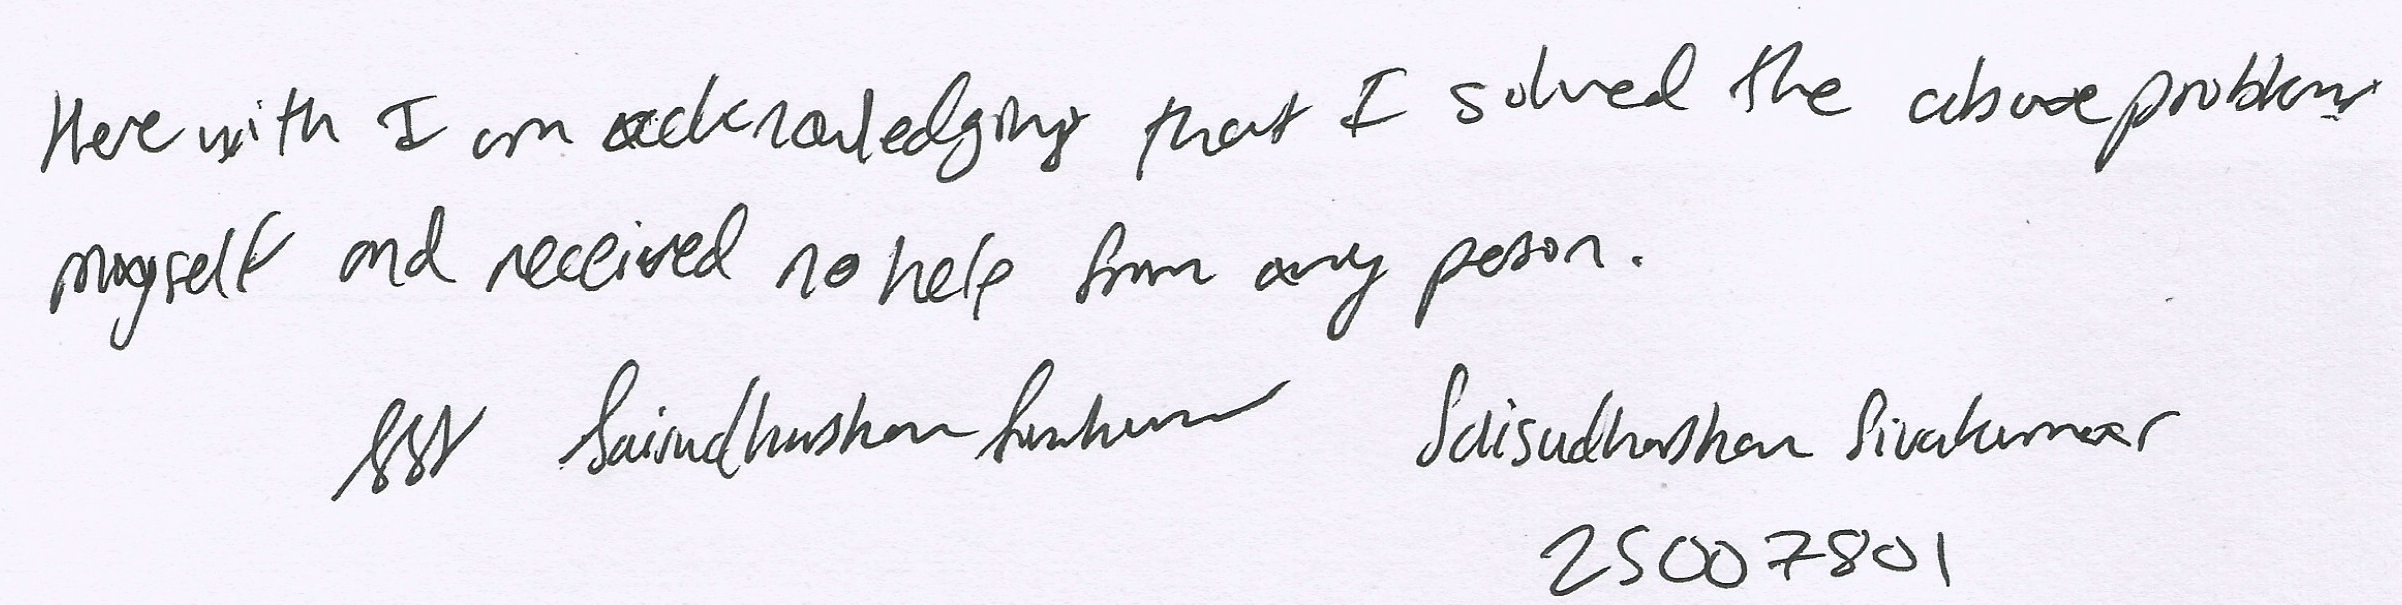
\includegraphics[scale=0.9]{signature}
%\end{figure}

\end{document}